\chapter{Implementação do método dos elementos virtuais para elementos unidimensionais sob esforços axiais}

\section{A equação diferencial unidimensional}

\indent Neste apêndice, é feita uma demonstração de como implementar o método dos elementos virtuais utilizando um exemplo numérico de uma treliça dinâmica. O objetivo é fornecer uma visão prática da aplicação do método, destacando os principais passos e considerações envolvidas na implementação.\\
\indent Para a implementação do modelo de exemplo é preciso adaptar a equação do movimento descrita no capítulo \ref{cap:3}, Eq. \ref{eq:3.1}, para um problema unidimensional. Simplificando os termos, chegamos à seguinte equação do movimento para uma treliça dinâmica:
\begin{equation} 
    EA\frac{d^2u}{dx^2} + f(x) = \rho A \frac{d^2u}{dt^2} 
\end{equation}
\indent Para solução do problema com o método dos elementos virtuais, é necessário que a equação diferencial seja convertida em uma forma integral, também conhecida como forma fraca. A forma fraca da equação do movimento é obtida multiplicando ambos os lados da equação por uma função de teste $v(x)$ e integrando sobre o domínio do problema:
\begin{equation}
    \int_{\Omega} EA\frac{d^2u}{dx^2} v(x) \, dx + \int_{\Omega} f(x) v(x) \, dx = \int_{\Omega} \rho A \frac{d^2u}{dt^2} v(x) \, dx.
\end{equation}
Nessa equação deve ser aplicada a integração por partes na parcela espacial para reduzir a ordem da derivada de $u(x)$, resultando na seguinte forma fraca:
\begin{equation}
    -\int_{\Omega} EA\frac{du}{dx} \frac{dv}{dx} \, dx + EA\frac{du}{dx} v(x) \Big|_{\partial \Omega} + \int_{\Omega} f(x) v(x) \, dx = \int_{\Omega} \rho A \frac{d^2u}{dt^2} v(x) \, dx.
\end{equation}
Reorganizando os termos, a forma fraca final da equação do movimento para a treliça dinâmica é:
\begin{equation}
    \int_{\Omega} EA\frac{du}{dx} \frac{dv}{dx} \, dx + \int_{\Omega} \rho A \frac{d^2u}{dt^2} v(x) \, dx = EA\frac{du}{dx} v(x) \Big|_{\partial \Omega} +\int_{\Omega} f(x) v(x) \, dx.
\end{equation}
\indent Métodos numéricos solucionam a equação diferencial para um conjunto finito de pontos, chamados de graus de liberdade, e as funções de base são utilizadas para interpolar os valores da função entre eles. Em um elemento de barra, os graus de liberdade são os deslocamentos nos nós do elemento e, particularmente para o MEV de alta ordem, os momentos internos.\\
\indent Assim como no Método dos Elementos Finitos, tanto a função de teste $v(x)$ quanto a função de deslocamento $u(x)$ são aproximadas por funções de base definidas em cada elemento do domínio. A aproximação da função de deslocamento $u(x)$ é expressa como uma combinação linear das funções de base $\varphi_i(x)$ ponderadas pelos graus de liberdade $u_i$:
\begin{equation}
    u(x) \approx \{\varphi(x)\}^T \{u^E\}.
\end{equation}
Assim como é feito no método de Galerkin, a função de teste $v(x)$ são aproximadas pelas funções de base do elemento. A forma discreta da equação do movimento para a treliça dinâmica é obtida substituindo as aproximações de $u(x)$ e $v(x)$ na forma fraca da equação do movimento:
\begin{equation}
    \begin{split}
        \int_{\Omega} EA \left(\frac{d}{dx}\{\varphi(x)\}^T\right) \frac{d}{dx}\{\varphi(x)\} \, dx \{u^E\} + \int_{\Omega} \rho A \{\varphi(x)\}^T \{\varphi(x)\} \, dx \, \{\ddot{u}^E\} = \\ EA\left(\frac{d}{dx}\{\varphi(x)\}^T\right) \{\varphi(x)\} \Big|_{\partial \Omega} + \int_{\Omega} f(x) \{\varphi(x)\} \, dx.
    \end{split}
\end{equation}
\indent As integrais da parcela esquerda da equação correspondem respectivamente as matrizes de rigidez e de massa, 
\begin{equation}
    K = \int_{\Omega} EA \left(\frac{d}{dx}\{\varphi(x)\}\right)^T \frac{d}{dx}\{\varphi(x)\} \, dx, \quad M = \int_{\Omega} \rho A \{\varphi(x)\}^T \{\varphi(x)\} \, dx,
\end{equation}
enquanto a parcela direita corresponde as forças externas. A partir dessa forma fraca, é possível aplicar o Método dos Elementos Virtuais para obter uma solução aproximada para o problema da treliça dinâmica.\\

\section{O Método dos Elementos Virtuais}

\indent Como visto na equação \ref{eq:4.3}, o MEV utiliza funções de base desconhecidas, mas mapeadas por uma projeção polinomial, separando a função de base em uma parcela polinomial e um complemento não polinomial. As matrizes de rigidez e de massa são então calculadas utilizando apenas a parcela polinomial da função de base, enquanto a parcela não polinomial é aproximada por um termo de estabilização das matrizes. Portanto, as matrizes de rigidez são descritas por:
\begin{equation}
    \begin{split}
        K = \int_{\Omega} EA \left(\frac{d}{dx}\Pi_k^{\Omega,\nabla}\{\varphi(x)\}^T\right) \frac{d}{dx}\Pi_k^{\Omega,\nabla}\{\varphi(x)\} \, dx + S_k, \\
        M = \int_{\Omega} \rho A \left(\frac{d^2}{dt^2}\Pi_k^{\Omega,0}\{\varphi(x)\}^T\right) \Pi_k^{\Omega,0}\{\varphi(x)\} \, dx + S_m,
    \end{split}
\end{equation}
com $S_k$ e $S_m$ sendo uma notação para as diferentes estabilizações abordadas no capítulo \ref{cap:4}. Diferente das matrizes de massa e rigidez, o termo de cargas não precisa do termo de estabilização, destarte:
\begin{equation}
    f_e = \int_{\Omega} f(x) \Pi_k^{\Omega,0} \{\varphi(x)\} \, dx.
\end{equation}
\indent Para os valores das integrais é necessário a obtenção dos projetores elíptico e $L^2$. Os projetores podem ser obtidos de diversas maneiras. Para se manter a consistência com o que foi apresentado no \ref{cap:4}, neste apêndice será realizada novamente a ortogonalização de uma função polinomial e outra não polinomial com a abordagem do método de Galerkin.

\subsection{Projetor elíptico}

\indent O projetor elíptico é utilizado para a aproximação das variações de primeira ordem das funções de base, e consequentemente da função das variáveis de campo. No contexto da mecânica estrutural o projetor elíptico é um mapa de funções polinomiais do campo de deformações do elemento ao invés dos deslocamentos. \\
\indent Como o operador diferencial da matriz de rigidez é uma derivada de primeira ordem, o projetor elíptico irá ortogonalizar as derivadas de uma função peso com a função resíduo obtida das funções de base.
\begin{equation}
    \begin{split}
        \int_{\Omega} \frac{d p_k(x)}{dx} \cdot \frac{d}{dx} \left( \varphi(x) - \Pi_k^{E,\nabla}\varphi(x) \right) dx = 0 \Rightarrow \\ 
        \int_{\Omega} \frac{d p_k(x)}{dx} \cdot \frac{d}{dx} \Pi_k^{E,\nabla}\varphi(x) dx = \int_{\Omega} \frac{d p_k(x)}{dx} \cdot \frac{d}{dx}\varphi(x)  dx \quad \forall \, p_k(x) \in \mathbb{P}_k(\Omega) 
    \end{split}
\end{equation}
\indent Por ser uma função polinomial, $\Pi_k^{E,\nabla}\varphi(x)$ pode ser escrito como a combinação linear de um vetor de bases polinomiais por um vetor de coeficientes para cada uma das funções de base. A função $p_k(x)$ é uma função polinomial qualquer, assim podendo assumir a forma de uma base polinomial, portanto:
\begin{equation}
     \int_{\Omega} \left(\frac{d}{dx} H_k(x)\right)^T \cdot \frac{d}{dx} H_k(x) \, dx \, \Pi_{k,*}^{\Omega,\nabla} = \int_{\Omega} \frac{d}{dx}H_k(x) \cdot \frac{d}{dx}\varphi(x) \, dx \Leftrightarrow \mathcal{G} \Pi_{k,*}^{\Omega,\nabla} = \mathcal{B}.
\end{equation}
\indent As integrais da matriz $\mathcal{G}$ em problemas unidimensionais podem ser avaliadas de maneira analítica para cada $k$. A matriz $\mathcal{B}$ deve ser separada em uma parcela do domínio e outra de contorno. Em problemas unidimensionais isso é feito utilizando integração por partes:
\begin{equation}
    \mathcal{B} = \left(\frac{d}{dx} H_k(x)\varphi(x)\right)\Big|_{0}^{l_e} - \int_{\Omega} \frac{d^2}{dx^2}H_k(x) \varphi(x) dx.
\end{equation}
Para aproximações com $k > 1$, os momentos internos são os valores de $\int_{\Omega} \frac{d^2}{dx^2}H_{k-2}(x) \varphi(x) dx$. 
\indent Diferente da formulação em duas dimensões, para elementos unidimensionais não são adicionados nós internos. Enquanto o contorno de um elemento bidimensional é composto por arestas, em elementos unidimensionais o contorno são os nós de vértice e o comprimento da barra equivale ao domínio. Então, serão utilizados momentos internos ao invés de nós de arestas tal qual o Método dos Elementos Finitos.\\
\indent Percebe-se que a primeira linha de ambas as matrizes $\mathcal{G}$ e $\mathcal{B}$ são nulas. Para isso aplica-se o projetor $P_0$, (Eq.~\ref{eq:4.32}), na primeira linha. O projetor elíptico se encontra na base polinomial. Para o termo de estabilização é necessário que ele esteja na base canônica. Desse modo avalia-se a matriz $\mathcal{D}$ através da equação \ref{eq:4.34}.

\vspace{5mm}
\noindent
\begin{tcolorbox}[breakable, colback=white, colframe=black, boxrule=0.4pt, arc=0pt, outer arc=0pt]
    \vspace{2mm} % Espaço interno superior
        \textbf{Exemplo C.1.} 
        
        \begin{enumerate}[label=\alph*), leftmargin=*]
            \item Calcule o projetor $\Pi^{\nabla}$ para uma interpolação de primeira ordem.
            \item Calcule o projetor $\Pi^{\nabla}$ para uma interpolação de segunda ordem.
            \item Calcule as matrizes $D$ para primeira e segunda ordem.
        \end{enumerate}
        
        \hrulefill

        Solução: 

        \begin{enumerate}[label=\alph*), leftmargin=*]
            \item O vetor $H_1(x)$ será, aqui, aproximado por monômios simples: $$H_1(x) = \begin{Bmatrix} 1 & x \end{Bmatrix}.$$ Assim a matriz $\mathcal{G}$ pode ser calculada:
            $$\begin{aligned}
                \mathcal{G} = \int_{0}^{l_e} \frac{d}{dx} \begin{Bmatrix} 1 \\ x \end{Bmatrix}  \cdot \frac{d}{dx} \begin{Bmatrix} 1 & x \end{Bmatrix} \, dx \, = \\
                \int_{0}^{l_e} \begin{Bmatrix} 0 \\ 1 \end{Bmatrix}  \cdot \frac{d}{dx} \begin{Bmatrix} 0 & 1 \end{Bmatrix} \, dx \, = \int_{0}^{l_e} \begin{Bmatrix} 0 & 0 \\ 0 & 1 \end{Bmatrix} \, dx \, = \mathcal{G} = \begin{Bmatrix} 0 & 0 \\ 0 & l_e \end{Bmatrix}.
            \end{aligned}$$
            Para a matriz $\mathcal{B}$ é necessário primeiro obter os polinômios de Lagrange correspondentes aos nós da barra: $$M_0(x) = \frac{(x - x_1)}{(x_0 - x_1)} = \frac{(x - l_e)}{(0 - l_e)} = - \frac{(x - l_e)}{l_e}$$ $$M_1(x) = \frac{(x - x_0)}{(x_1 - x_0)} = \frac{(x - 0)}{(l_e - 0)} = \frac{x}{l_e}.$$ Calculadas as funções de forma da barra\footnote{Contra intuitivo, eu sei. Tudo pela didática.}, a matriz $\mathcal{B}$ pode ser calculada:
            $$\begin{aligned}
                \mathcal{B} = \left(\frac{d}{dx} \begin{Bmatrix} 1 \\ x \end{Bmatrix}\varphi(x)\Big|_{\partial \Omega}\right)\Big|_{0}^{l_e} - \int_{\Omega} \frac{d^2}{dx^2}\begin{Bmatrix} 1 \\ x \end{Bmatrix} \varphi(x) dx = \left( \begin{Bmatrix} 0 \\ 1 \end{Bmatrix}\begin{Bmatrix} M_0 & M_1 \end{Bmatrix}\right)\Big|_{0}^{l_e} = \\
                \left( \begin{bmatrix} 0 & 0 \\ M_0(x) & M_1(x) \end{bmatrix}\right)\Big|_{0}^{l_e} = \begin{bmatrix} 0 & 0 \\ M_0(l_e) & M_1(l_e) \end{bmatrix} - \begin{bmatrix} 0 & 0 \\ M_0(0) & M_1(0) \end{bmatrix} =\\
                \begin{bmatrix} 0 & 0 \\ M_0(l_e) - M_0(0) & M_1(l_e) - M_1(0) \end{bmatrix} = \begin{bmatrix} 0 & 0 \\ -1 & 1 \end{bmatrix}.
            \end{aligned}$$
            $$\mathcal{G} = \begin{bmatrix} 2 & l \\ 0 & l_e \end{bmatrix} \quad \mathcal{B} = \begin{bmatrix} 1 & 1 \\ 1 & 1 \end{bmatrix}.$$
            Conhecidas $\mathcal{G}$ e $\mathcal{B}$ calcula-se o projetor elíptico na base polinomial: $$\Pi_{1,*}^{\Omega,\nabla} = \mathcal{G}^{-1} \mathcal{B} = \frac{1}{l_e} \begin{bmatrix} l_e  & 0 \\ -1 & 1 \end{bmatrix}.$$
            \vspace{2mm}
            \item O processo de cálculo é o mesmo que $k=1$, todavia as matrizes terão dimensões maiores, a matriz $H_k(x)$ é $H_2(x) = \begin{bmatrix} 1 & x & x^2 \end{bmatrix}$ e haverá um momento interno. A matriz $\mathcal{G}$ será calculada do mesmo modo que $k=1$, portanto o resultado é: $$\mathcal{G} = \begin{bmatrix} 0 & 0 & 0 \\ 0 & l & l^2 \\ 0 & l^2 & \frac{4l^3}{3} \end{bmatrix}.$$
            \indent Desenvolvendo $\mathcal{B}$: 
            $$\begin{aligned} \mathcal{B} = \left(\frac{d}{dx} \begin{Bmatrix} 1 \\ x \\ x^2 \end{Bmatrix}\varphi(x)\Big|_{\partial \Omega}\right)\Big|_{0}^{l_e} - \int_{\Omega} \frac{d^2}{dx^2}\begin{Bmatrix} 1 \\ x \\ x^2 \end{Bmatrix} \varphi(x) dx = \\
            \left( \begin{Bmatrix} 0 \\ 1 \\ 2x \end{Bmatrix}\begin{Bmatrix} M_0 & M_1 & 0 \end{Bmatrix}\right)\Big|_{0}^{l_e} - \int_{\Omega} \begin{Bmatrix} 0 \\ 0 \\ 2 \end{Bmatrix}\begin{Bmatrix} 0 & 0 & M_3 \end{Bmatrix} dx = \\
            \left( \begin{bmatrix} 0 & 0 & 0 \\ M_0(x) & M_1(x) & 0 \\ 2xM_0(x) & 2xM_1(x) & 0 \end{bmatrix}\right)\Big|_{0}^{l_e} - \begin{bmatrix} 0 & 0 & 0 \\ 0 & 0 & 0 \\ 0 & 0 & 2l_e M_3 \end{bmatrix} = \\
            \begin{bmatrix} 0 & 0 & 0 \\ M_0(l_e) & M_1(l_e) & 0 \\ 2xM_0(l_e) & 2xM_1(l_e) & 0  \end{bmatrix} - \begin{bmatrix} 0 & 0 & 0 \\ M_0(0) & M_1(0) & 0 \\ 2xM_0(0) & 2xM_1(0) & 0  \end{bmatrix} - \begin{bmatrix} 0 & 0 & 0 \\ 0 & 0 & 0 \\ 0 & 0 & 2l_e M_3 \end{bmatrix} = \\
            \begin{bmatrix} 0 & 0 & 0 \\ M_0(l_e) - M_0(0) & M_1(l_e) - M_1(0) & 0 \\ 0 & 2l_e & - 2l_eM_3 \end{bmatrix} = \begin{bmatrix} 0 & 0 & 0 \\ -1 & 1 & 0 \\ 0 & 2l_e & - 2l_e \end{bmatrix}.
            \end{aligned}$$
            \indent Os diferentes vetores de $\varphi$ estão relacionados ao contorno e domínio. Na parcela de contorno $M_3$ não entra porque ele é uma variável interna do elemento, ao passo que na integral de domínio $M_0$ e $M_1$ são nulos. Apesar das funções de forma terem sido desenvolvidas com o polinômio de Lagrange, elas se comportam como deltas de Kronecker.\\
            \indent De maneira análoga ao caso $k=1$, é necessário a aplicação do projetor $P_0$ na primeira linha das matrizes $\mathcal{B}$ e $\mathcal{G}$:
            $$\mathcal{G} = \begin{bmatrix} 1 & \frac{l}{2} & \frac{l^2}{3} \\ 0 & l & l^2 \\ 0 & l^2 & \frac{4l^3}{3} \end{bmatrix} \quad \mathcal{B} = \begin{bmatrix} 0 & 0 & 1 \\ -1 & 1 & 0 \\ 0 & 2l_e & - 2l_e \end{bmatrix}.$$
            E, portanto, o projetor:
            $$\Pi_{2,*}^{\Omega,\nabla} = \begin{bmatrix} 1 & 0 & 0 \\ -\frac{4}{l_e} & -\frac{2}{l_e} & \frac{6}{l_e} \\ \frac{3}{l_e^2} & \frac{3}{l_e^2} & -\frac{6}{l_e^2} \end{bmatrix}.$$
            \vspace{2mm}
            \item Calcule as matrizes $D$ para primeira e segunda ordem.
            $$\mathcal{D} = \chi (p_1) = \begin{bmatrix} 1 & 0 \\ 1 & l_e \end{bmatrix}.$$
            $$\mathcal{D} = \chi (p_2) =  \begin{bmatrix} 1 & 0 & 0 \\ 1 & l_e & l^2 \\ 1 & \frac{l}{2} & \frac{l^2}{3} \end{bmatrix}.$$
        \end{enumerate}
        
        \vspace{2mm} % Espaço interno inferior
\end{tcolorbox}
\vspace{5mm}

\indent Um fenômeno a ser notado é o projetor elíptico na base canônica para problemas unidimensionais ser equivalente à matriz identidade: $$\Pi_k^{\Omega,\nabla} = \Pi_{k,*}^{\Omega,\nabla} \mathcal{D}$$
\begin{equation}
    \Pi_1^{\Omega,\nabla} = \begin{bmatrix} 1 & 0 \\ 0 & 1 \end{bmatrix} \quad \Pi_2^{\Omega,\nabla} = \begin{bmatrix} 1 & 0 & 0 \\ 0 & 1 & 0 \\ 0 & 0 & 1 \end{bmatrix}.
\end{equation}
Uma implicação desse fenômeno é o termo não polinomial ser nulo para problemas unidimensionais. 


\subsection{Projetor $L^2$-ortogonal}

\indent O projetor $L^2$ foi desenvolvido para atuar junto aos termos da equação diferencial em sua forma fraca que não possuam operadores diferenciais na integral. Esse operador utilizada um espaço expandido como visto no capítulo \ref{cap:4}. Diferente do operador elíptico, o operador $L^2$ aplica ortogonaliza diretamente os campos de deslocamentos, ou seja, não são aplicados operadores diferenciais as funções de base. Aplicando o método de Galerkin:
\begin{equation}
    \int_0^{l_e} p_k(x) \cdot (\varphi - \Pi_k^{\Omega,0}\varphi) \, dx = 0 \Rightarrow \int_0^{l_e} p_k(x) \cdot \Pi_k^{\Omega,0}\varphi \, dx = \int_0^{l_e} p_k(x) \cdot \varphi \, dx \quad \forall \, p_k(x) \in \mathbb{P}_k(\Omega).
\end{equation}
\indent Substituindo $p_k(x)$ e $\Pi_k^{\Omega,0}\varphi$ pela base polinomial:
\begin{equation}
    \int_0^{l_e} H_k(x) \cdot H_k(x) \, dx \Pi_k^{\Omega,0} = \int_0^{l_e} H_k(x) \cdot \varphi \, dx \Leftrightarrow \mathcal{H} \Pi_k^{\Omega,0} = \mathcal{Q}.
\end{equation}
A matriz $\mathcal{H}$ é calculada da mesma forma que $\mathcal{G}$. Para a matriz $\mathcal{Q}$ segue a fórmula apresentada na equação \ref{eq:4.43}, mas com os limites reduzidos, pois os graus de liberdade são escalares, assim, o limite de $2n_{k-2}$ passa a ser apenas $n_{k-2}$ e $2n_k$ se torna $n_k$.

\vspace{5mm}
\noindent
    \begin{tcolorbox}[breakable, colback=white, colframe=black, boxrule=0.4pt, arc=0pt, outer arc=0pt]
        \vspace{2mm} % Espaço interno superior
        \textbf{Exemplo C.2.} 
        
        \begin{enumerate}[label=\alph*), leftmargin=*]
            \item Calcule o projetor $\Pi^{0}$ para uma interpolação de primeira ordem.
            \item Calcule o projetor $\Pi^{0}$ para uma interpolação de segunda ordem.
        \end{enumerate}
        
        \hrulefill

        Solução: 
        \vspace{2mm}

        \begin{enumerate}[label=\alph*), leftmargin=*]
            \item Para $k=1$ a matriz $\mathcal{H}$ é: $$\mathcal{H} = \begin{bmatrix} \int_0^{l_e} 1 \cdot 1 \, dx & \int_0^{l_e} 1 \cdot x \, dx \\ \int_0^{l_e} x \cdot 1 \, dx & \int_0^{l_e} x \cdot x \, dx \end{bmatrix} = \begin{bmatrix} l_e &  \frac{l_e^2}{2} \\ \frac{l_e^2}{2} & \frac{l_e^3}{3} \end{bmatrix}.$$
            Como não há momentos internos, a matriz $\mathcal{Q}$ é obtida diretamente da integral do produto de $p_k(x)$ com $\Pi_{k,*}^{\Omega,\nabla}$:
            $$\mathcal{Q} = \int_0^{l_e} p_k(x) \cdot \Pi_k^{\Omega,\nabla}\varphi \, dx = \int_0^{l_e} H_k(x) \cdot H_k(x) \, dx \Pi_k^{\Omega,\nabla} \Rightarrow \mathcal{Q} = \mathcal{H}\Pi_k^{\Omega,\nabla} = \begin{bmatrix} \frac{l_e}{2} &  \frac{l_e}{2} \\ \frac{l_e^2}{6} & \frac{l_e^2}{3} \end{bmatrix}.$$
            \indent Com $\mathcal{H}$ e  $\mathcal{Q}$ computa-se o projetor $\Pi_{1,*}^{\Omega,0}$:
            $$\Pi_{1,*}^{\Omega,0} = \mathcal{H}^{-1} \mathcal{Q} = \frac{1}{l_e} \begin{bmatrix} l_e & 0 \\ -1 & 1 \end{bmatrix}.$$
            \vspace{2mm}
            
            \item A principal diferença entre os casos $k=1$ e $k=2$ está na presença dos momentos internos. A avaliação da matriz $\mathcal{H}$ será apenas uma extensão de $k=1$:
            $$\mathcal{H} = \begin{bmatrix} \int_0^{l_e} 1 \cdot 1 \, dx & \int_0^{l_e} 1 \cdot x \, dx & \int_0^{l_e} 1 \cdot x^2 \, dx \\ \int_0^{l_e} x \cdot 1 \, dx & \int_0^{l_e} x \cdot x \, dx & \int_0^{l_e} x \cdot x^2 \, dx \\ \int_0^{l_e} x^2 \cdot 1 \, dx & \int_0^{l_e} x~2 \cdot x \, dx & \int_0^{l_e} x^2 \cdot x^2 \, dx \end{bmatrix} = \begin{bmatrix} l_e &  \frac{l_e^2}{2} & \frac{l_e^3}{3} \\ \frac{l_e^2}{2} & \frac{l_e^3}{3} & \frac{l_e^4}{4} \\ \frac{l_e^3}{3} & \frac{l_e^4}{4} & \frac{l_e^5}{5} \end{bmatrix}.$$
            \indent Com a presença dos momentos internos, a primeira linha de $\mathcal{Q}$ será calculada de maneira diferente das demais. A primeira linha é nula e a coluna correspondente ao momento interno é igual ao comprimento da barra, enquanto as demais utilizam o teorema dos projetores equivalentes. Para a primeira linha:
            $$\mathcal{Q}_{1i} = \begin{bmatrix} 0 & 0 & l_e \end{bmatrix}.$$
            Para as demais linhas:
            $$\mathcal{Q}_{\alpha i} = \left(\mathcal{H}\Pi_k^{\Omega,\nabla}\right)_{\alpha i} = \begin{bmatrix} -\frac{l_e^2}{12} & \frac{l_e^2}{12} & \frac{l_e^2}{2} \\ -\frac{l_e^3}{15} & \frac{l_e^3}{10} & \frac{3l_e^3}{10}  \end{bmatrix}.$$
            \indent O projetor para o caso $k=2$ é:
            $$ \Pi_{2,*}^{\Omega,0} = \mathcal{H}^{-1} \mathcal{Q} = \begin{bmatrix} 1 & 0 & 0 \\ -\frac{4}{l_e} & -\frac{2}{l_e} & \frac{6}{l_e} \\ \frac{3}{l_e^2} & \frac{3}{l_e^2} & -\frac{6}{l_e^2} \end{bmatrix}.$$
        \end{enumerate}
        
        \vspace{2mm} % Espaço interno inferior
    \end{tcolorbox}
\vspace{5mm}

\indent Nota-se que para problemas unidimensionais os projetores $\Pi_{k,*}^{\Omega,\nabla}$ e $\Pi_{k,*}^{\Omega,0}$ são exatamente iguais para ambos os casos $k=1$ e $k=2$.

\subsection{Matrizes de massa e rigidez}

\indent No método dos elementos virtuais, tanto a matriz de massa quanto a matriz de rigidez são separadas em uma parcela de consistência contendo apenas os termos polinomiais de ordem $k$ e uma segunda parcela não polinomial. Como visto na secção anterior, o termo de estabilização é nulo em problemas unidimensionais sob esforços axiais, assim, a formulação só utiliza o termo de consistência. \\
\indent A aproximação da parcela de consistência da matriz de rigidez é feita utilizando o projetor elíptico. Considerando os valores do módulo de elasticidade e da área constantes, a matriz de rigidez consistente é:
\begin{equation}
    \begin{split}
        K = EA \int_{0}^{l_e} \left(\frac{d}{dx}\{\Pi_{k}^{\nabla} \varphi(x)\}^T\right) \frac{d}{dx}\{\Pi_{k}^{\nabla} \varphi(x)\} \, dx = \\
        EA \int_{0}^{l_e} \left(\frac{d}{dx}\{H_k(x) \Pi_{k,*}^{\Omega,\nabla} \}^T\right) \frac{d}{dx}\{H_k(x) \Pi_{k,*}^{\Omega,\nabla}\} \, dx = \\
        EA \left(\Pi_{k,*}^{\Omega,\nabla}\right)^T \int_{0}^{l_e} \left(\frac{d H_k(x)}{dx}\right)^T \frac{d H_k(x)}{dx} \, dx \, \Pi_{k,*}^{\Omega,\nabla}.
    \end{split}
\end{equation}


\vspace{5mm}
\noindent
    \begin{tcolorbox}[breakable, colback=white, colframe=black, boxrule=0.4pt, arc=0pt, outer arc=0pt]
        \vspace{2mm} % Espaço interno superior
        \textbf{Exemplo C.3.} 
        
        \begin{enumerate}[label=\alph*), leftmargin=*]
            \item Calcule a matriz de rigidez utilizando os projetores de primeira ordem.
            \item Calcule a matriz de rigidez utilizando os projetores de segunda ordem.
        \end{enumerate}
        
        \hrulefill

        Solução: 
        \vspace{2mm}

        \begin{enumerate}[label=\alph*), leftmargin=*]
            \item Para o vetor de bases polinomiais e os projetores elípticos quando $k=1$:
            $$\begin{aligned}
                K = EA \left(\begin{bmatrix} l_e  & 0 \\ -1 & 1 \end{bmatrix}\right)^T \int_{0}^{l_e} \frac{d}{dx}\begin{Bmatrix} 1 \\ x \end{Bmatrix} \cdot \frac{d}{dx}\begin{Bmatrix} 1 & x \end{Bmatrix} \, dx \, \begin{bmatrix} l_e  & 0 \\ -1 & 1 \end{bmatrix} = \\
                EA \left(\begin{bmatrix} l_e  & 0 \\ -1 & 1 \end{bmatrix}\right)^T \begin{bmatrix} 0  & 0 \\ 0 & l_e \end{bmatrix}  \begin{bmatrix} l_e  & 0 \\ -1 & 1 \end{bmatrix} = \frac{EA}{l_e} \begin{bmatrix} 1 & -1 \\ -1 & 1 \end{bmatrix}
            \end{aligned}$$
            
            \vspace{2mm}
            
            \item Quando $k=2$:
            $$\begin{aligned}
                K = EA \left(\begin{bmatrix} 1 & 0 & 0 \\ -\frac{4}{l_e} & -\frac{2}{l_e} & \frac{6}{l_e} \\ \frac{3}{l_e^2} & \frac{3}{l_e^2} & -\frac{6}{l_e^2} \end{bmatrix}\right)^T \int_{0}^{l_e} \frac{d}{dx}\begin{Bmatrix} 1 \\ x \\ x^2 \end{Bmatrix} \cdot \frac{d}{dx}\begin{Bmatrix} 1 & x & x^2 \end{Bmatrix} \, dx \, \begin{bmatrix} 1 & 0 & 0 \\ -\frac{4}{l_e} & -\frac{2}{l_e} & \frac{6}{l_e} \\ \frac{3}{l_e^2} & \frac{3}{l_e^2} & -\frac{6}{l_e^2} \end{bmatrix} = \\
                EA \left(\begin{bmatrix} 1 & 0 & 0 \\ -\frac{4}{l_e} & -\frac{2}{l_e} & \frac{6}{l_e} \\ \frac{3}{l_e^2} & \frac{3}{l_e^2} & -\frac{6}{l_e^2} \end{bmatrix}\right)^T \begin{bmatrix} 0  & 0 & 0 \\ 0 & l_e & l_e^2 \\ 0 & l_e^2 & \frac{4l_e^3}{3} \end{bmatrix}  \begin{bmatrix} 1 & 0 & 0 \\ -\frac{4}{l_e} & -\frac{2}{l_e} & \frac{6}{l_e} \\ \frac{3}{l_e^2} & \frac{3}{l_e^2} & -\frac{6}{l_e^2} \end{bmatrix} = \frac{EA}{l_e} \begin{bmatrix} 4 & 2 & -6 \\ 2 & 4 & -6 \\ -6 & -6 & 12 \end{bmatrix}
            \end{aligned}$$
        \end{enumerate}
        
        \vspace{2mm} % Espaço interno inferior
    \end{tcolorbox}
\vspace{5mm}

\indent Observa-se que a matriz de rigidez utilizando o método dos elementos virtuais é a mesma que a do método dos elementos finitos. \\
\indent O cálculo da matriz de massa é feito de maneira análoga ao da matriz de rigidez. Nos casos bi e tridimensionais utiliza-se o projetor $L^2$-ortogonal visto que não há operadores diferenciais dentro da integral. Porém, como foi visto nos exemplos numéricos dos projetores, tanto o projetor elíptico quanto o $L^2$ são idênticos para o caso unidimensional. A matriz de massa para $\rho$ e $A$ constantes:
\begin{equation}
    \begin{split}
        M = \rho A \int_{0}^{l_e} \left(\Pi_{k}^{0}\{\varphi(x)\}\right)^T \Pi_{k}^{0}\{\varphi(x)\} \, dx \, = \\
        \rho A \int_{0}^{l_e} \left(\Pi_{k}^{\Omega,0} H_k(x)\right)^T \Pi_{k}^{\Omega,0}H_k(x) \, dx \, = \\
        \rho A  \left(\Pi_{k}^{\Omega,0}\right)^T \int_{0}^{l_e} \left(H_k(x)\right)^T H_k(x) \, dx \,\Pi_{k}^{\Omega,0}.
    \end{split}
\end{equation}

\vspace{5mm}
\noindent
    \begin{tcolorbox}[breakable, colback=white, colframe=black, boxrule=0.4pt, arc=0pt, outer arc=0pt]
        \vspace{2mm} % Espaço interno superior
        \textbf{Exemplo C.4.} 
        
        \begin{enumerate}[label=\alph*), leftmargin=*]
            \item Calcule a matriz de massa utilizando os projetores de primeira ordem.
            \item Calcule a matriz de massa utilizando os projetores de segunda ordem.
        \end{enumerate}
        
        \hrulefill

        Solução: 
        \vspace{2mm}

        \begin{enumerate}[label=\alph*), leftmargin=*]
            \item Para a matriz de massa com $\rho$ e $A$ constantes:
            $$\begin{aligned}
                M = \rho A  \left(\begin{bmatrix} l_e  & 0 \\ -1 & 1 \end{bmatrix}\right)^T \int_{0}^{l_e}  \begin{Bmatrix} 1 \\ x \end{Bmatrix} \begin{Bmatrix} 1 & x \end{Bmatrix}(x) \, dx \,\begin{bmatrix} l_e  & 0 \\ -1 & 1 \end{bmatrix} = \\
                \rho A \left(\begin{bmatrix} l_e  & 0 \\ -1 & 1 \end{bmatrix}\right)^T \begin{bmatrix} l_e  & \frac{l_e^2}{2} \\ \frac{l_E^2}{2} & \frac{l_e^3}{3} \end{bmatrix} \, \begin{bmatrix} l_e  & 0 \\ -1 & 1 \end{bmatrix} = \rho A l_e^3 \begin{bmatrix} \frac{1}{3} & \frac{1}{6} \\ \frac{1}{3} & \frac{1}{6} \end{bmatrix}.
            \end{aligned}$$
            
            \vspace{2mm}
            
            \item Caso $k=2$:
            $$\begin{aligned}
                M = \rho A  \left(\begin{bmatrix} 1 & 0 & 0 \\ -\frac{4}{l_e} & -\frac{2}{l_e} & \frac{6}{l_e} \\ \frac{3}{l_e^2} & \frac{3}{l_e^2} & -\frac{6}{l_e^2} \end{bmatrix}\right)^T \int_{0}^{l_e}  \begin{Bmatrix} 1 \\ x \\ x^2 \end{Bmatrix} \begin{Bmatrix} 1 & x & x^2 \end{Bmatrix}(x) \, dx \,\begin{bmatrix} 1 & 0 & 0 \\ -\frac{4}{l_e} & -\frac{2}{l_e} & \frac{6}{l_e} \\ \frac{3}{l_e^2} & \frac{3}{l_e^2} & -\frac{6}{l_e^2} \end{bmatrix} = \\
                \rho A \left(\begin{bmatrix} 1 & 0 & 0 \\ -\frac{4}{l_e} & -\frac{2}{l_e} & \frac{6}{l_e} \\ \frac{3}{l_e^2} & \frac{3}{l_e^2} & -\frac{6}{l_e^2} \end{bmatrix}\right)^T \begin{bmatrix} l_e  & \frac{l_e^2}{2} & \frac{l_e^3}{3} \\ \frac{l_E^2}{2} & \frac{l_e^3}{3} & \frac{l_e^4}{4} \\ \frac{l_E^3}{3} & \frac{l_e^4}{4} & \frac{l_e^5}{5} \end{bmatrix} \, \begin{bmatrix} 1 & 0 & 0 \\ -\frac{4}{l_e} & -\frac{2}{l_e} & \frac{6}{l_e} \\ \frac{3}{l_e^2} & \frac{3}{l_e^2} & -\frac{6}{l_e^2} \end{bmatrix} = \frac{\rho A l_e}{5} \begin{bmatrix} \frac{2}{3} & -\frac{1}{6} & -\frac{1}{2} \\ -\frac{1}{6} & \frac{2}{3} & -\frac{1}{2} \\ -\frac{1}{2} & -\frac{1}{2} & 6 \end{bmatrix}.
            \end{aligned}$$
        \end{enumerate}
        
        \vspace{2mm} % Espaço interno inferior
    \end{tcolorbox}
\vspace{5mm}

\section{Montagem das matrizes de rigidez e massa globais}

\indent Cada elemento possui uma matriz de rigidez e massa contendo os graus de liberdade do elemento. Para a solução do problema é preciso que as matrizes elementares sejam alocadas em uma matriz global que contem todos os graus de liberdade do sistema:
\begin{equation}
    \mathbf{K} = \bigcup_{e=1}^{n_{el}} \mathbf{K}_e  \quad \mathbf{M} = \bigcup_{e=1}^{n_{el}} \mathbf{M}_e 
\end{equation}
\indent Para exemplificar o problema uma viga em balanço é modelada como um elemento de barra e discretizada em dois elementos, figura~\ref{fig:C.1}. Para efeito de cálculo a secção transversal com área e módulo de elasticidade constantes.
\begin{figure}[H]
    \centering
    \caption{Viga em balanço com lateral esquerda engastada discretizada em dois elementos.}
    \label{fig:C.1}
    \resizebox{0.6\textwidth}{!}{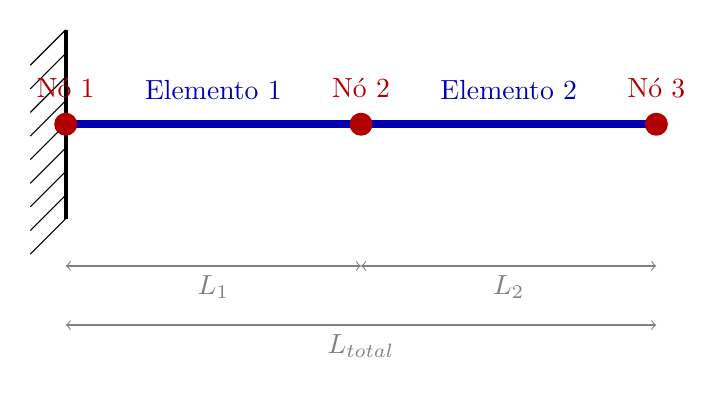
\begin{tikzpicture}[scale=1.5, thick]
    % Coordenadas dos Nós
    \coordinate (N1) at (0,0);
    \coordinate (N2) at (2.5,0);
    \coordinate (N3) at (5,0);

    % Engaste na esquerda (Nó 1)
    \draw[line width=1.5pt] (0,-0.8) -- (0,0.8);
    \foreach \y in {-0.8,-0.6,...,0.8}
        \draw[thin] (0,\y) -- (-0.3,\y-0.3);

    % Elementos Finitos da Viga
    \draw[line width=3pt, blue!70!black] (N1) -- (N2) node[midway, above=4pt] {Elemento 1};
    \draw[line width=3pt, blue!70!black] (N2) -- (N3) node[midway, above=4pt] {Elemento 2};

    % Nós e Rótulos dos Nós
    \filldraw[red!70!black] (N1) circle (2.5pt) node[above=6pt] {Nó 1};
    \filldraw[red!70!black] (N2) circle (2.5pt) node[above=6pt] {Nó 2};
    \filldraw[red!70!black] (N3) circle (2.5pt) node[above=6pt] {Nó 3};

    % Linhas de cota e comprimentos
    \draw[<->, thin, gray] (0,-1.2) -- (2.5,-1.2) node[midway, below] {$L_1$};
    \draw[<->, thin, gray] (2.5,-1.2) -- (5,-1.2) node[midway, below] {$L_2$};
    \draw[<->, thin, gray] (0,-1.7) -- (5,-1.7) node[midway, below] {$L_{total}$};
\end{tikzpicture}}
\end{figure}
\indent Para uma aproximação de primeira ordem, as matrizes de rigidez e massa do primeiro elementos são respectivamente:
\begin{equation}
    K_1 = \frac{EA}{L_1} \begin{bmatrix} 1 & -1 \\ -1 & 1 \end{bmatrix} \quad M_1 = \rho A L_1^3 \begin{bmatrix} \frac{1}{3} & \frac{1}{6} \\ \frac{1}{3} & \frac{1}{6} \end{bmatrix}.
\end{equation}
Para o segundo elemento:
\begin{equation}
    K_2 = \frac{EA}{L_2} \begin{bmatrix} 1 & -1 \\ -1 & 1 \end{bmatrix} \quad M_2 = \rho A L_2^3 \begin{bmatrix} \frac{1}{3} & \frac{1}{6} \\ \frac{1}{3} & \frac{1}{6} \end{bmatrix}.
\end{equation}
\indent O primeiro passo para a montagem das matrizes globais é a identificação da conectividade dos nós dos elementos. O elemento 1 possui os nós 1 e 2, e, o elemento 2 os nós 2 e 3. O nó 1 possui deslocamento nulo. Para montagem da matriz de rigidez global, as matrizes elementares podem ser convertidas para um sistema global através da construção de matrizes de incidência cinemática. \\
\indent Para a construção da matriz de incidência cinemática, cria-se uma matriz com número de linhas igual à quantidade de graus de liberdade do elemento e o número de colunas é a quantidade de graus de liberdade do sistema. Todos os valores da matriz são zero com exceção do componente grau de liberdade que vale 1. Para os elementos 1 e 2 as matrizes de incidência cinemática são:
\begin{equation}
    IC_{1} = \begin{bmatrix} 1 & 0 & 0 \\ 0 & 1 & 0 \end{bmatrix} \quad IC_{2} = \begin{bmatrix} 0 & 1 & 0 \\ 0 & 0 & 1 \end{bmatrix}.
\end{equation}
\indent A conversão das matrizes do elemento 1 são feitas por:
\begin{equation}
    K = \sum_{i = 1}^{n_{elem}} IC_{i}^T K_i IC_{i}  \quad M = \sum_{i = 1}^{n_{elem}} IC_{i}^T M_i IC_{i}
\end{equation}
\indent A matriz global é obtida somando todos os elementos:
\begin{equation}
    K = EA \begin{bmatrix} \frac{1}{L_1} & -\frac{1}{L_1} & 0 \\ -\frac{1}{L_1} & \frac{(L_1 + L_2)}{L_1L_2} & -\frac{1}{L_2} \\ 0 & -\frac{1}{L_2} & \frac{1}{L_2} \end{bmatrix} \quad
    M = \frac{\rho A}{3} \begin{bmatrix}  L_1^3 & \frac{L_1^3}{2} & 0 \\ L_1^3 & \frac{(L_1^3 + 2L_2^3)}{2} & \frac{L_2^3}{2} \\ 0 &  L_2^3 & \frac{ L_2^3}{2}  \end{bmatrix}
\end{equation}
